\documentclass{acm_proc_article-sp}


\usepackage{listings}
\usepackage[T1]{fontenc}
%\usepackage[utf8]{inputenc}
%\usepackage{amsmath}
%\usepackage{amssymb}
%\usepackage[usenames]{color}
%\usepackage{graphicx}
%\usepackage{url}
%\usepackage[scaled=0.8]{luximono}

%\usepackage{hyperref}
%\usepackage[compact]{titlesec}
%\usepackage[small]{caption}
%\usepackage{tikz}
%\usetikzlibrary{matrix,chains,scopes,positioning,arrows,fit}


% ----- begin macros
\lstdefinelanguage{Scala}%
{morekeywords={abstract,%
  case,catch,char,class,%
  def,else,extends,final,for,%
  if,import,implicit,%
  match,module,%
  new,null,%
  object,override,%
  package,private,protected,public,%
  for,public,return,super,%
  this,throw,trait,try,type,%
  val,var,%
  with,while,%
  yield%
  },%
  sensitive,%
  morecomment=[l]//,%
  morecomment=[s]{/*}{*/},%
  morestring=[b]",%
  morestring=[b]',%
  showstringspaces=false%
}[keywords,comments,strings]%

\lstset{language=Scala,%
  mathescape=true,%
%  columns=[c]fixed,%
%  basewidth={0.5em, 0.40em},%
  aboveskip=1pt,%\smallskipamount,
  belowskip=1pt,%\negsmallskipamount,
  lineskip=-0.2pt,
  basewidth={0.54em, 0.4em},%
  basicstyle=\ttfamily,%\scriptsize,%
  keywordstyle=\bfseries%\sffamily\bfseries,%
%  keywordstyle=\sffamily\bfseries,%
%  xleftmargin=0.5cm
}

\lstnewenvironment{listing}{\lstset{language=Scala}}{}
\newcommand{\scode}[1]{\lstinline[language=Scala,columns=fixed,basicstyle=\ttfamily]|#1|}
\newcommand{\jcode}[1]{\lstinline[language=Java,flexiblecolumns=true,basicstyle=\ttfamily]{#1}}
\newcommand{\code}[1]{\scode{#1}}

\newcommand{\todo}[1]{{\color{red} \bf [TODO: #1 ]}}
\newcommand{\commentstyle}[1]{\slseries{#1}}
\newcommand{\keywordstyle}[1]{\bfseries{#1}}
\newcommand{\comment}[1]{}
\newcommand{\note}[1]{$\spadesuit$ \textbf{#1} $\clubsuit$}
\graphicspath{{figures/}}

\setlength{\floatsep}{2pt plus 2pt minus 2pt}
\setlength{\textfloatsep}{2pt plus 2pt minus 2pt}
\setlength{\intextsep}{2pt plus 2pt minus 2pt}
\setlength{\dblfloatsep}{2pt plus 2pt minus 2pt}
\setlength{\dbltextfloatsep}{2pt plus 2pt minus 2pt}
%\setlength{\bibsep}{0.0pt}

% Packed item, so we don't waste space
\newenvironment{sitemize}{
\begin{itemize}
  \setlength{\itemsep}{1pt}
  \setlength{\parskip}{0pt}
  \setlength{\parsep}{0pt}
}{\end{itemize}}
% ----- end macros

\raggedbottom

\begin{document}
  %\conferenceinfo{BigData'12,} {(date and location)}
  %\CopyrightYear{2012}
  %\copyrightdata{(provided by acm)}

  %
  % Title
  % 
    
  \title{Stivo: Embedded DSL for High Performance BigData Processing}
  %\subtitle{[Extended Abstract]
  %\titlenote{A full version of this paper is available as
  %\textit{Author's Guide to Preparing ACM SIG Proceedings Using
  %\LaTeX$2_\epsilon$\ and BibTeX} at
  %\texttt{www.acm.org/eaddress.htm}} 


  %
  % Authors
  % 
  \numberofauthors{1} 
  \author{
	% 1st. author
	\alignauthor
	Ben Trovato\titlenote{Dr.~Trovato insisted his name be first.}\\
	 %\affaddr{Institute for Clarity in Documentation}\\
	 %\affaddr{1932 Wallamaloo Lane}\\
	 %\affaddr{Wallamaloo, New Zealand}\\
	 %\email{trovato@corporation.com}
        % \and for another row of authors 
  }
  
%  \additionalauthors{Additional authors: John Smith (The Th{\o}rv{\"a}ld Group,
%	email: {\texttt{jsmith@affiliation.org}}) and Julius P.~Kumquat
%	(The Kumquat Consortium, email: {\texttt{jpkumquat@consortium.net}}).}
  
  
  
  \date{22 May 2012}
  \maketitle
  
  \begin{abstract}
    Cluster computing systems today impose a trade-off between generality,
performance and productivity. Hadoop and Dryad force programmers to write low
level programs that are tedious to compose but easy to optimize. Systems like
Dryad/LINQ and Spark allow concise modeling of user programs but do not apply
relational optimizations. Pig and Hive restrict the language to achieve
relational optimizations, making complex programs hard to express without user
extensions. However, these extensions are cumbersome to write and disallow
program optimizations.

We present a distributed batch data processing framework called \tool.
\tool uses deep language embedding in Scala, multi-stage programming and
explicit side effect tracking to analyze the structure of user programs. The
analysis is used to apply projection insertion, which eliminates unused data, as
well as code motion and operation fusion to highly optimize the performance
critical path of the program. The language embedding and a high-level interface
allow \tool programs to be both expressive, resembling regular Scala code, and
optimized. Its modular design allows users to extend \tool with modules that
produce highly performant code. Through a modular code generation scheme, \tool
can generate programs for both Spark and Hadoop. Compared with na\"{\i}ve
implementations we achieve 143\% speedups on Spark and 126\% on Hadoop.

  \end{abstract}
  
  %\category{D.1.3}{Programming Techniques}{Concurrent Programming -- Parallel programming}
  %\category{D.3.3}{Programming Languages}{Language Constructs and Features -- Concurrent programming structures}
  %\category{D.3.4}{Programming Languages}{Processors -- Code generation, Optimization, Run-time environments}
  %\terms Design, Languages
  %\keywords Code Generation, Multi-stage programming, Domain-specific languages, Language Virtualization


  %
  % Sections 
  %
  \section{Introduction}
\label{sec:introduction}

% Motivation -- three different types programming models and their problems
In the past decade, numerous systems for big data cluster computing have been studied \cite{dean_mapreduce:_2008, yu_dryadlinq:_2008-1, olston_pig_2008-1, thusoo_hive_2010-1, spark-nsdi}. Programming models of these systems impose a trade-off between generality, performance and productivity. Systems like Hadoop MapReduce, \cite{hadoop} and Dryad \cite{isard_dryad:_2007} provide a low level general purpose programming model that allows writing fine grained and optimized code. However, low level optimizations greatly sacrifice productivity \cite{chambers_flumejava:_2010}. Restricted programming models like Pig latin \cite{olston_pig_2008-1} exploit domain knowledge to provide both good performance and productivity for a large number of use cases. However, they support generality only through user defined functions that are cumbersome and difficult to optimize. Finally, models like Spark \cite{spark-nsdi}, FlumeJava \cite{chambers_flumejava:_2010} and Dryad/LINQ \cite{yu_dryadlinq:_2008-1} provide high level operations and general purpose programming models, but their performance is limited by glue code between high level operations. Also, many relational optimizations are impossible due to the lack of knowledge about the program structure. 

% Trade-off - why cant there be both generality, performance and productivity
Above mentioned trade-off exists due to the imperative programming models, run-time binding of methods and open world assumptions commonly used in languages for big data processing. This limits compiler's ability to optimize the code. Inefficient abstractions like iterators and channels are not removed from the code that connects declarative operations. Side effect free operations like date/time instantiation, regular expression compilation and high precision decimal numbers are often hidden by abstraction and recomputed in the hot path for each piece of data. 

Domain specific approaches, like Pig and SQL, have a narrow and side effect free interface and provide good optimizations. However, they come with their own set of limitations. Their programming model is often too simple for the problem. This requires reverting to external language operations, which are again hard to optimize, or to abandoning the model completely. Moreover, there is the high overhead of learning the new language and proper tool support debugging, type driven correctness checking and IDE support is often limited. Also it is hard to extend these frameworks with optimizations for a new domain.

% Existing Solutions to achieve this
In the recent history there have been several solutions that try to make programming big data systems efficient, productive and general at the same time. Steno \cite{murray_steno:_2011} implements an innovative runtime code generation scheme that eliminates iterators in Dryad/LINQ queries. It operates over flat and nested queries and produces a minimal number of loops without any iterator calls. Manimal \cite{jahani_automatic_2011} and HadoopToSQL \cite{iu_hadooptosql:_2010} apply byte code analysis to extract information about unused data columns and selection conditions to gain enough knowledge to apply common relational database optimizations for projection and selection. However, since these solutions use static byte code analysis they must be safely conservative which can lead to missed optimization opportunities.

% general, restricted
% optimizations
% modular/extensible
% portable
This paper presents a new domain specific language \tool for big data processing that provides a high level declarative interface similar to Dryad/LINQ and Spark. \tool builds upon language virtualization \cite{moors_scala-virtualized_2012} and lightweight modular staging \cite{rompf_lightweight_2010} (LMS) and has the same syntax and semantics as the regular Scala language with only a few restrictions.
Because \tool includes common compiler and relational optimizations, as well as domain specific ones, it produces very fast programs. It is designed in a very modular way - the code generation is completely independent of the parsing and optimizations - and allows extensions for supported operations, optimizations and backends. 
% Our implementation

% Contributions
\tool makes following contributions to the state of the art:    
\begin{itemize}

  \item We implement the \tool framework for big data processing. \tool has a high level programming model with carefully chosen restrictions that allow relational, domain specific and compiler optimizations but do not sacrifice generality.
%  \item \todo{link generality to optimizations}We implement the \tool framework for big data processing. \tool has a slightly restricted and high level programming model but still applies relational, domain specific and compiler optimizations to achieve high performance.

  \item We introduce a novel projection insertion algorithm that operates across general program constructs like classes, conditionals, loops and user defined functions, takes the whole program into account and does not rely on safe assumptions which lead to missed optimization opportunities.  

  \item We show that \tool allows easy language extension and code portability for big data frameworks. 

\end{itemize} 

% Sections
In section \ref{sec:background} we will provide background on LMS, language virtualization and big data frameworks. Then, in section \ref{sec:programming-model} we explain the programming model and present simple program examples. In section \ref{sec:optimizations} we explain the novel projection insertion optimization algorithm in section \ref{sec:field-reduction} and section \ref{sec:fusion} explains the fusion optimization. We evaluate \tool in \ref{sec:evaluation} and discuss our approach in section \ref{sec:discussion}. \tool is compared to state of the art in section \ref{sec:related-work}, future work is in section \ref{sec:future-work} and we conclude in section \ref{sec:conclusion}.

  \section{Evaluation}
\label{sec:evaluation}

We evaluate \tool by implementing a word count program with prior text parsing, TPCH query 12 and a k-means application that uses array processing extension for \tool. \\

All experiments were performed on the Amazon EC2 Cloud, using 20 "m1.large" nodes as slaves and one as master. They each have 7.5 Gb of memory, 2 virtual cores with 2 EC2 compute units each, have 850 Gb of instance storage and provide high throughput. Prior to the experiments we have measured up to 50 MB/s between two nodes. For the Hadoop experiments we used current Clouderas Hadoop distribution cdh3u4. We used Crunch version 0.2.4 and Scoobi 0.4.0. We did not tweak Hadoop configuration beyond the default settings. For benchmarking Spark we used the Mesos \cite{hindman_mesos:_2011} EC2 script to start a cluster, and then most recent version of Spark for our tests.  For Spark we changed the default parallelism level to the number of machines in the cluster and increased the available memory to 6GB. 

% Regular expressions
For a fairer comparison with Pig we adapted some of their regular expression optimizations for our program. Pig makes use of a faster library \todo{cite brics.automaton} and implements an optimized splitting function when the regular expression becomes a simple comparison of one character. We implemented a frontend for regular expressions which automatically selects the best variant for each expression and operation. 

We were also getting unsatisfying numbers from our Scoobi backend, so we added Crunch with about one week of effort. This really shows that it is easy to implement a new backend, and the modularity allows us to reuse pieces of other backends. Crunch's implementation of join performed very badly in local benchmarks, so we replaced it with our own one for these benchmarks.

% Data Serialization
For serialization of data we used LMS code generation to achieve minimal overhead for both Crunch and Scoobi frameworks. We used generated versions since they outperformed the Kryo framework by a thin margin. For Spark we used Kryo. All benchmarks were run three times and in the figures we present only the average. We also measured standard deviation but it is not displayed since it is smaller than 3\% of the job time in all experiments.

\begin{figure}[!hbt]
    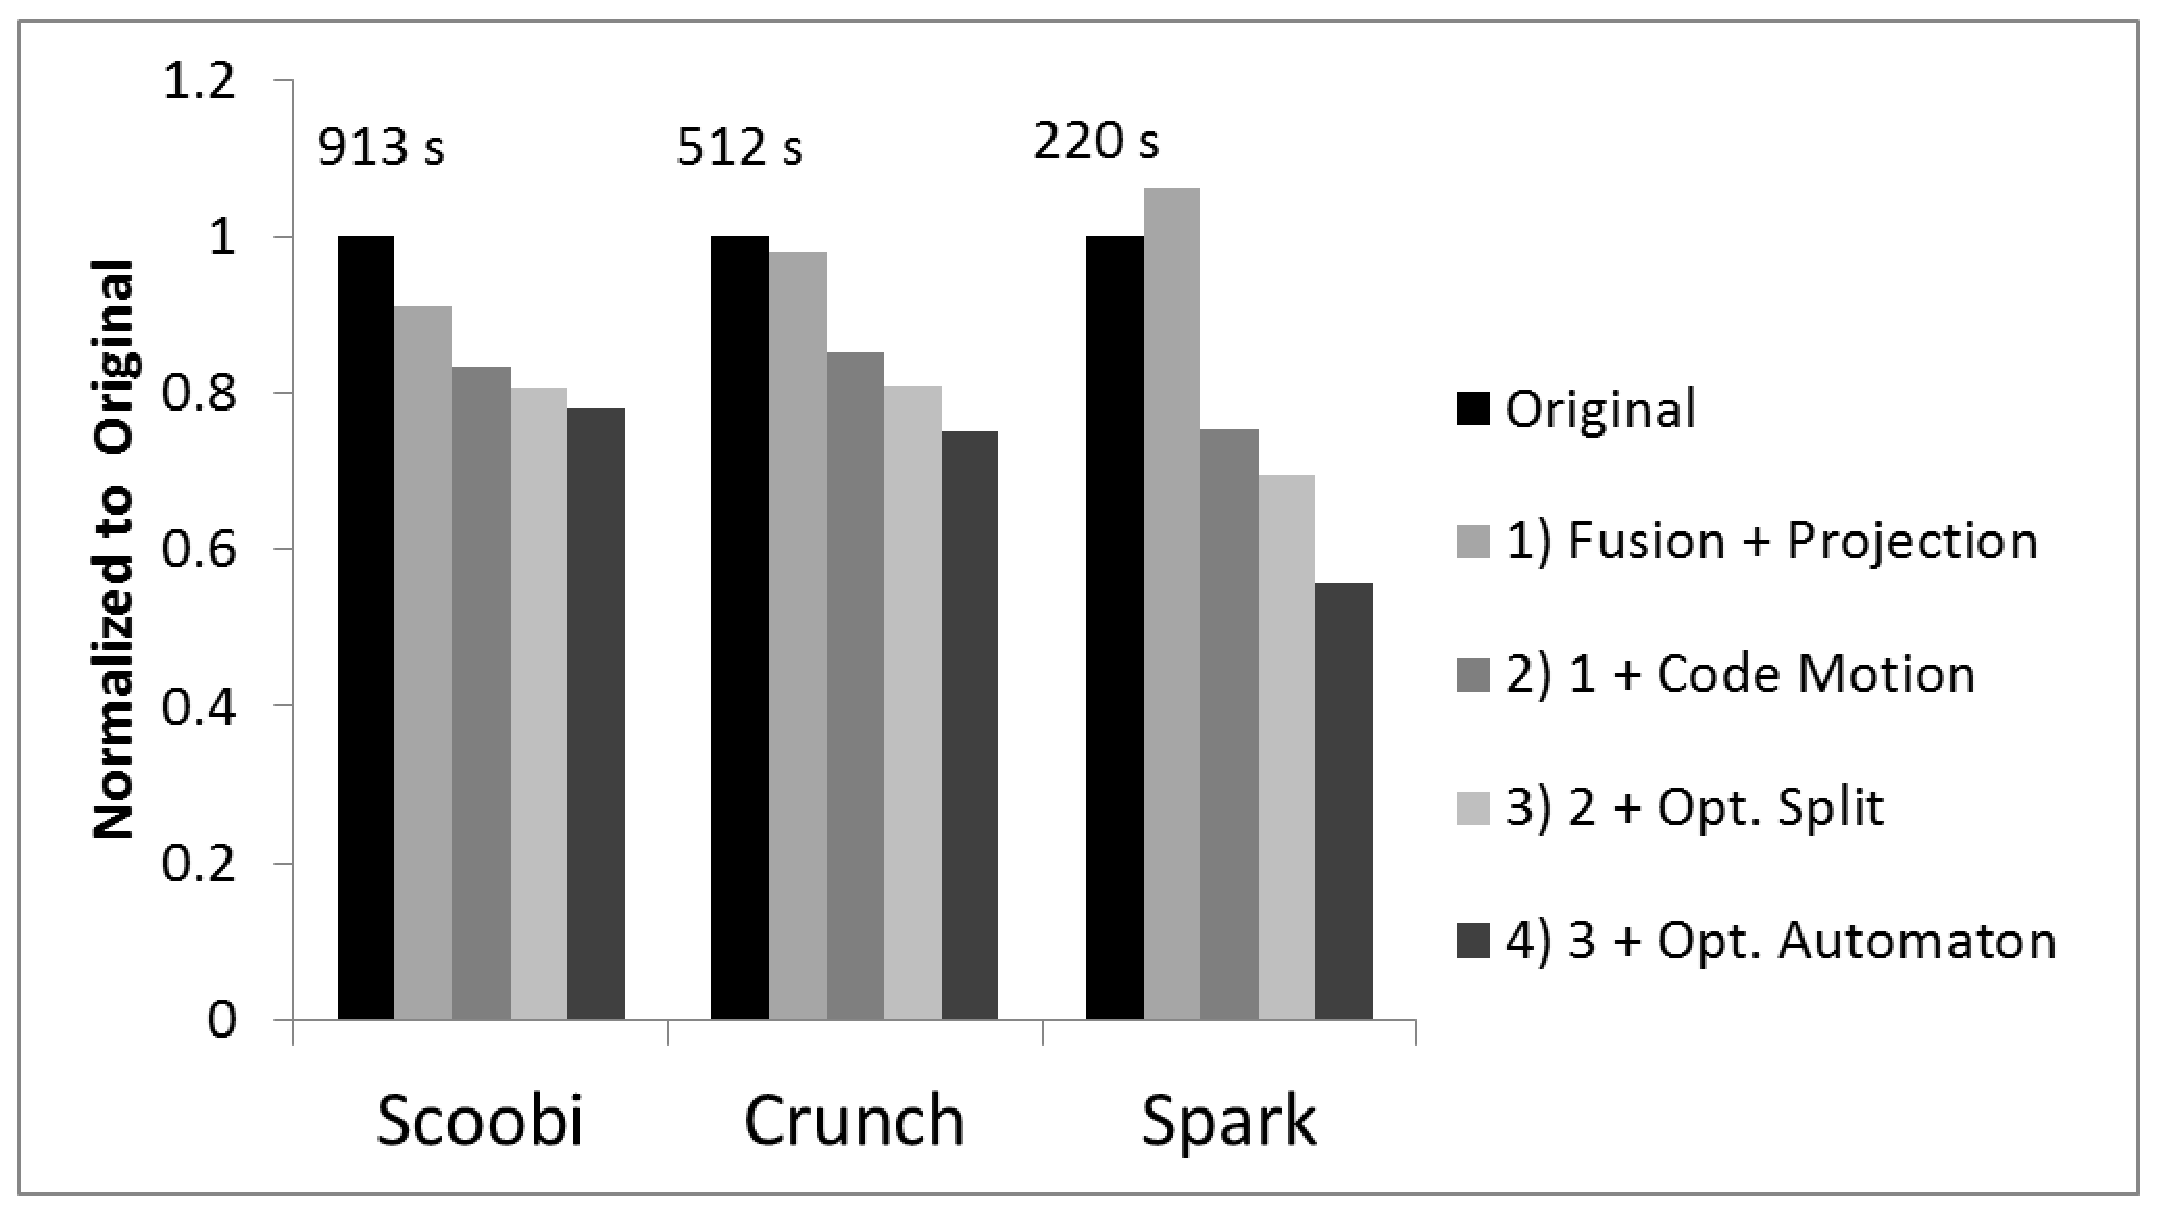
\includegraphics[width=8.6cm]{figures/word-count}
    \label{fig:word-count}\\%\vspace{10pt}
   \caption{Word Count benchmark.}
\end{figure}

\begin{figure}[!hbt]
    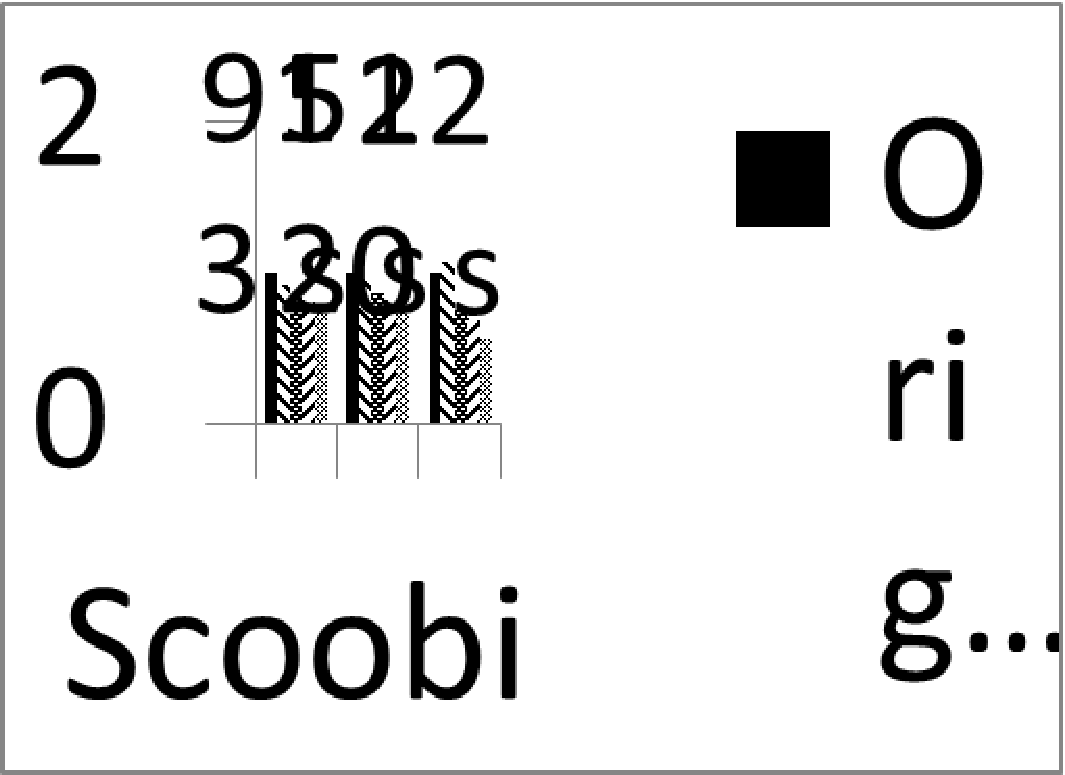
\includegraphics[width=8.6cm]{figures/k-means}
    \label{fig:k-means}\\%\vspace{10pt}
   \caption{K-means benchmark.}
\end{figure}

\begin{figure}[!hbt]
    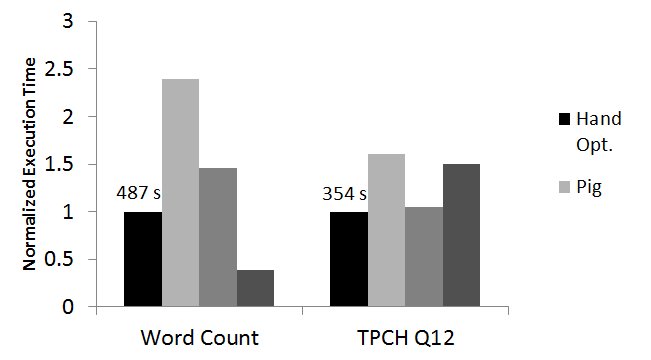
\includegraphics[width=8.6cm]{figures/pig}
    \label{fig:pig}\\%\vspace{10pt}
   \caption{Comparison with Pig.}
\end{figure}

\begin{figure}[!hbt]
    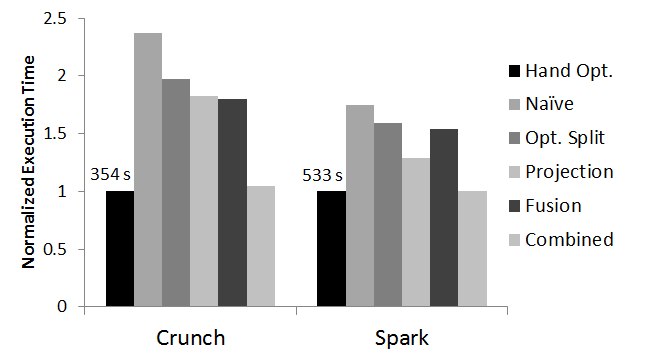
\includegraphics[width=8.6cm]{figures/tpch}
    \label{fig:tpch}\\%\vspace{10pt}
   \caption{TPCH query 12 benchmark.}
\end{figure}

% WordCount
\subsection{Parsing and Word Count}
\label{subsec:parsing-word-count}
\todo{Stivo explain the regular expressions and what do we want to prove}
Our input is a 62 Gb set of freebase wikipedia data. As the data in that example is not entirely cleaned up we use regular expressions to filter out words and to split it in a custom manner. Our program uses 5 regular expressions in total which are quite expensive and we are certain that this is a cpu-bound program, such that our optimizations become relevant.
It can not benefit from field reduction and it only requires one shuffle stage, so its performance is dependant on the cpu time on the mapper side. 

For this evaluation we start with an unoptimized version and add optimizations one by one. We first add our loop fusion and field reduction optimizations. Then we reuse the patterns instead of recompiling them. Next we add the fast splitter and for the fully optimized version we add the faster regex library. 

In figure \ref{fig:word-count} we show the job times for these versions normalized to the unoptimized program version. In this benchmark we notice that code motion removes regular expressions automaton compilation from the hot loop. Performance improvements are from \todo{75-82} in Scoobi, \todo{Crunch} and in Spark. Also, we notice significant fusion increase in Scoobi which indicates that the framework imposes additional overhead for declarative operations. 

In Spark, we notice larger benefits from optimizations. We believe that it has significantly smaller IO overhead so that the optimizations have a bigger effect. Also, we notice that fusion optimization and field reduction is slower than the original program, but only in Spark. This result does not match our experiments in a smaller cluster setup. We believe that it could be caused by a straggler node in the cloud environment.

% TPCH q12
\subsection{TPCH Query 12}
\label{subsec:tpch-query-12}

To evaluate effects of projection insertion we have run the TPCH query 12 which includes an expensive \code{join} operation and aggregates the whole result to just two values. As the data set we use a 100 GB input data set generated by the DbGen generator \cite{_dbgen_????}.

In figure \ref{fig:tpch} we show job times for different optimizations normalized to the unoptimized program version on different frameworks. We notice that projection insertion gives 20\% percent better performance on Crunch and 11\% on Scoobi. On Spark projection insertion gives significantly better improvements than on Hadoop based frameworks. We believe that either network shuffle or the \code{join} operation are less optimal in Spark. In this benchmark absolute performance gain for combined optimizations is 3\% greater for Crunch, the equal to for Scoobi and 9\% smaller for Spark than sum of absolute individual gains. 

\subsection{Comparison with Pig}
\label{subsec:pig}
% Pig Comparison

In figure \ref{fig:pig} we compare most optimal versions of benchmarks to equivalent Pig programs. The figure is normalized to the Pig execution time and overall job time is stated above the bar. We notice that for TPCH query 12, combination of fusion, code motion and field reduction outperform Pig when the Crunch framework is used. For Crunch, field reduction alone is not enough to outperform the Pig framework. We believe that this result is caused by more efficient join operation in Pig. In future work we will investigate the cause for this.
In the Word Count Crunch outperforms Pig even without any optimizations applied. With all optimizations the difference is significant. We explain this by the more optimal regular expressions processing support included in \tool. In regular expressions used in the benchmark Pig falls back to default Java regular expressions while \tool uses optimized automaton library. Scoobi framework performs slower than Pig in both benchmarks even with all optimizations applied.

\todo{go up}
For the sake of showing comparison between the Hadoop based frameworks and the Spark framework we include the Spark results in the graph. We see that in all cases except for unoptimized TPCH query 12 it significantly outperforms Hadoop based frameworks.

\subsection{K-Means}
\label{subsec:kmeans}
\todo{Stivo KMeans graph explanation}
\todo{this section needs to point out interactivity}

% KMeans
We took a version of Spark k-means program \todo{cite NSDI} application and ported it to our own language. This application can neither use field reduction nor can it really profit from loop fusion. We extended our DSL for this program with a highly optimized vector type that has all operations compiled into while loops. As this program uses operations only available in Spark, and it has been shown that Spark outperforms Hadoop by a large margin for it, we have only benchmarked it against the original Spark implementation. As input we use synthetic data with 10 to 1000 dimensions, 100 centers and we keep the dimensions * points factor constant at 2000000000, such that each input file is around 20Gb. 

Our results are similar to those described by Murray and al. in Steno\cite{}. In lower dimensions our optimization shows an impressive speedup while at 1000 dimensions our version performs slightly worse. We believe that the iterator overhead is quite high for 10 dimensions, such that our loops which removes it performs much better. At higher dimensions it's possible that the JVM can do a better job optimizing if the code is smaller, such that our pre optimized and larger code becomes slightly slower. In any case our implementation seems favorable as it performs more consistently for different dimensions.

  \section{Related Work}
\label{sec:related-work}



  \section{Conclusion}
\label{sec:conclusion}

We have presented the distributed batch data processing framework \tool that provides an
expressive high-level programming model. \tool uses language virtualization,
lightweight modular staging and side effect tracking to analyze user programs at
runtime. This allows \tool to apply projection insertion, code motion as well as
operation fusion optimizations to achieve high performance for declarative
programs. Through modular code generation \tool allows execution on Spark and
Crunch. Presented optimizations result in speedups of up to 143\% in
Spark and up to 126\% in Crunch.

Unlike existing domain-specific approaches \tool provides high-performance,
a general and expressive programming model which is integrated into the Scala
language. It allows high performance user extensions and provides code
portability between different distributed batch data processing frameworks.
%\PB

  
  %
  % Bibliography
  %
  
  % Defined by the template
  \bibliographystyle{abbrv}
  \bibliography{vjovanov-lib}

\end{document}
